%--------------------------------
%SUB - MÉTODO
\section{Method}
\label{cap5_metodologia}

The project architecture uses VGG16 neural network with multiple side-outputs, in order to obtain multi-level features.
It proposes to train the network without forcing side-outputs to produce similar predictions, to reduce the number of training iterations.
The architectures here are inspired by HED \cite{HED:2015} and RCF \cite{RCF:2017:8100105} networks.

%--------------------------------
%SUB - TÉCNICAS PARA COMBINAR SAÍDAS laterais
\subsection{Neural Network Architecture}
\label{cap5_rede_neural}

VGG16's architecture is made up of 13 convolutional layers, divided into 5 stages, with 2 or 3 convolutional layers.
It uses a rectified linear unit $ReLU(\cdot) = max(0, \cdot)$ as an activation function and a max-pooling layer.
At the end of the network, it has a fully connected layer, a ReLU layer and a final layer with the softmax activation function, totaling 16 weight layers \cite{VGGNET:2014}.

% \begin{figure}
%   \centering
%   \caption{VGG16's architecture.}
%   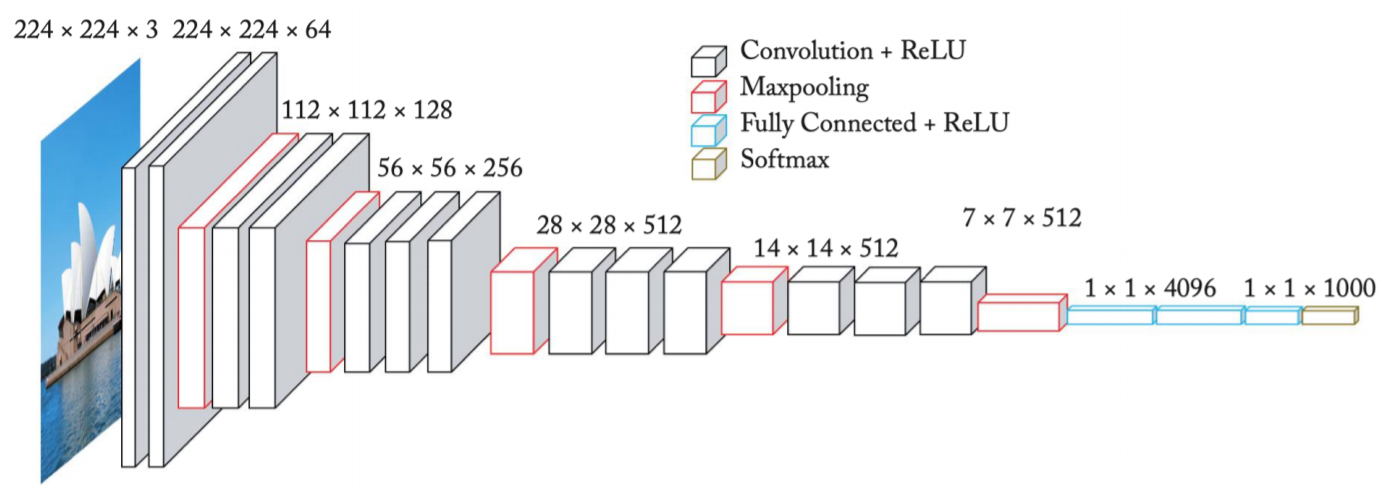
\includegraphics[width=0.8\textwidth]{../../imagens/ilustracoes/cap5_vgg16.png}
%   \par \textbf{Source: \cite{Cao:2020}, based on \cite{VGGNET:2014}.}
%   \label{fig:architecture_vgg16}
% \end{figure}

%The work developed here followed the approaches present in the networks  HED \cite{HED:2015} and RCF \cite{RCF:2017:8100105}, which make changes in the final layers to build their architectures.
To build our architecture, the last activation layer and all the fully connected layers of the VGG16 network were removed.
Also it was added side-outputs in different quantities, for evaluation.
In the first proposal, side-outputs were added in the last convolution of each stage, while in the second, secondary outputs were added after each convolutional layer.
Details regarding these architectures, influence on training and accuracy will be discussed in Sections \ref{cap5_saidas_laterais} and \ref{cap6_experm_1_qtd_saidas}.
An overview of the architecture can be seen in Figure \ref{fig:method}.

VGG16 was chosen due its overall performance and its relatively simplicity to create, train and study the influence of side-outputs, being suitable for our experiments. 
Creating, training and analyzing the influence of outputs is a simpler task than in residual networks such as ResNet \cite{RESNET:2016:7780459}, despite its higher performance.

%--------------------------------
%SUB - INFLUÊNCIA DO NÚMERO DE SAÍDAS laterais
\subsection{Side-outputs}
\label{cap5_saidas_laterais}

In addition to following the VGG16 architecture, the work used side-outputs, like several other existing approaches described in Section \ref{cap4_trab_rel}.
To evaluate the most appropriate number of side-outputs, it was analyzed HED and RCF architectures.
HED creates outputs after the last convolutional layer of each stage (5 outputs), while RCF adds side-outputs after each of the convolutions (13 outputs) \cite{HED:2015} \cite{RCF:2017:8100105}.

The first strategy, named \textit{Stage Layer Outputs} (\textbf{SLO}) and inspired by the HED model, creates a side-output $\mathcal{H}_i$ for each stage $S$ of the network.
Its graphical representation is available in Figure \ref{fig:architecture_slo}.
The second strategy, named \textit{All Layers Outputs} (\textbf{ALO}) and inspired by the RCF architecture, creates a side-output $\mathcal{H}_i$ for each convolutional layer $L$, as detailed in Figure \ref{fig:architecture_alo}.

\begin{figure*}
  \centering
  \caption{SLO Neural Network Architecture.}
  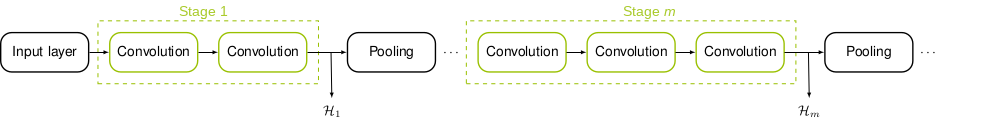
\includegraphics[width=0.7\textwidth]{../../imagens/ilustracoes/cap6_arquitetura_slo.png}
  \sourceOwn
  \label{fig:architecture_slo}
\end{figure*}

\begin{figure*}
  \centering
  \caption{ALO Neural Network Architecture.}
  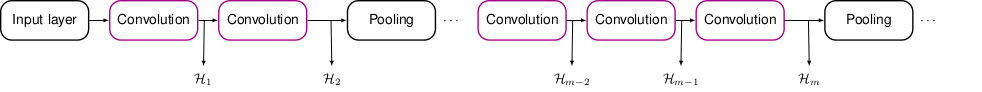
\includegraphics[width=0.7\textwidth]{../../imagens/ilustracoes/cap6_arquitetura_alo.png}
  \sourceOwn
  \label{fig:architecture_alo}
\end{figure*}

% \begin{figure}
%   \centering
%   \caption{SLO Neural Network Architecture.}
%   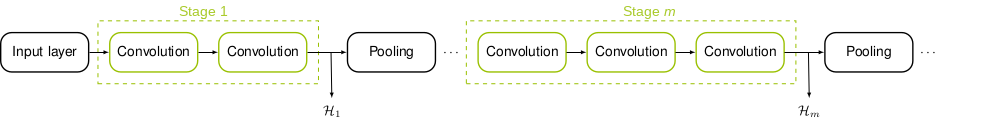
\includegraphics[width=1\columnwidth]{../../imagens/ilustracoes/cap6_arquitetura_slo.png}
%   \sourceOwn
%   \label{fig:architecture_slo}
% \end{figure}
% 
% \begin{figure}
%   \centering
%   \caption{ALO Neural Network Architecture.}
%   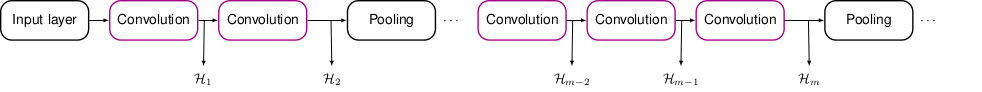
\includegraphics[width=1\columnwidth]{../../imagens/ilustracoes/cap6_arquitetura_alo.png}
%   \sourceOwn
%   \label{fig:architecture_alo}
% \end{figure}

In SLO, the number of side-outputs corresponds to the number of network stages $|S|$.
In turn, in the ALO method, the amount of output equals the number of convolutional layers $|L|$.
Formally, the set $ \mathcal{H}$ of $m$ side-outputs maps in each strategy is defined as:

\begin{align}
\mathcal{H}_{SLO}=\{\mathcal{H}_1,...,\mathcal{H}_m~|&~ m \le |S|\}\\
\mathcal{H}_{ALO}=\{\mathcal{H}_1,...,\mathcal{H}_m~|&~ m \le |L|\}
\end{align}

Each side-output $\mathcal{H}_1, ... \mathcal{H}_m$ is composed of a $1 \times 1$ convolution, followed by a transposed convolution of variable size.
Due to the network architecture, with \textit{pooling} layers, the images are reduced along the network. 
Thus, for the images to be resized to a single size, it is necessary that the transposed convolutions have a variable size.
%The evaluation of the learning curve and final post-training performance of each strategy will be presented in Section \ref{cap6_experm_1_qtd_saidas}.

%--------------------------------
%SUB - TÉCNICAS PARA COMBINAR SAÍDAS LATERAIS
\subsection{Side-outputs Merging Techniques}
\label{cap5_func_combinar_saidas}

Working with side-outputs requires that methods be used to combine intermediate results.
These are generated at different scales and may represent different concepts due to the position of the output on the network.
The goal, then, is to produce a single proposition $\hat{Y}$ to be evaluated in the task, keeping useful information contained in different layers.

In this work, a new strategy is developed to overcome the challenge of combining the outputs by exploring the knowledge of the learning process.
Operations are performed element-wise at each side-output.
To do this, the initial step is to resize the images generated at different stages of the network, so that they all have the same size.
Then, different trivial merge functions were studied and compared, once each of these has an expected behavior, as described below:

\begin{itemize}
  %\itemsep0.1cm
  \item \textit{ADD}: sums intermediate results, aiming to balance negative and positive weights;
  \item \textit{AVG}: calculates the average value of the outputs to create a proposal that represents learning at all levels;
  \item \textit{MAX}: returns the maximum value between the results, aiming to value the most confident outputs.
\end{itemize}

Formally, the combined output $\mathcal{Z}$ in each strategy can be defined as:

\begin{align}
  \mathcal{Z}_{ADD} &= \sum_{i=1}^{m}(\mathcal{H}_i)\\
  \mathcal{Z}_{AVG} &= \frac{\sum_{i=1}^{m}(\mathcal{H}_i)}{m}\\
  \mathcal{Z}_{MAX} &= \max_{1 \leq i \leq m} (\mathcal{H}_i)
\end{align} 

%--------------------------------
\subsection{Merged Output}
\label{cap5_saida_final_rede}

After combining the side-outputs as detailed in Section \ref{cap5_func_combinar_saidas}, a single final prediction $\hat{Y}$ is produced.
The value is obtained by executing a convolutional operation of $1 \times 1$ followed by a ReLU activation function.
The method overview is illustrated in Figure \ref{fig:method}.

\begin{figure*}
  \centering
  \caption{Overview of our method.}
  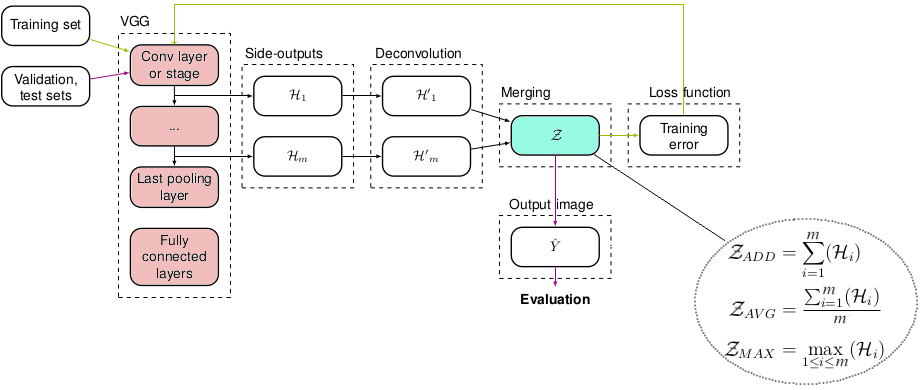
\includegraphics[width=0.7\textwidth]{../../imagens/ilustracoes/cap5_metodo.png}
  \sourceOwn
  \label{fig:method}
\end{figure*}

% \begin{figure}
%   \centering
%   \caption{Overview of our method.}
%   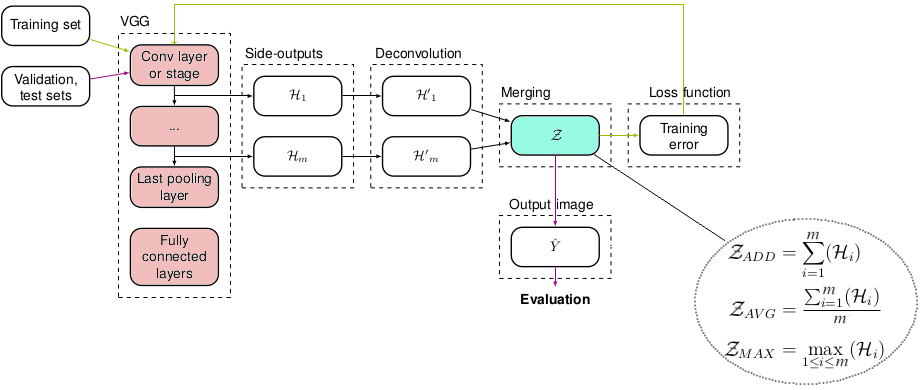
\includegraphics[width=1\columnwidth]{../../imagens/ilustracoes/cap5_metodo.png}
%   \sourceOwn
%   \label{fig:method}
% \end{figure}

In region segmentation tasks, $\hat{Y}$ seeks to provide partitions that represent significant areas of an image, while in the edge detection tasks, it seeks to represent the boundary between regions.

\begin{comment}
Na tarefa de segmentação multirregiões, a proposição $\hat{Y}$ pode ser reduzida a um problema binário.
Nele, objetivo seria distinguir cada pixel da imagem como pertencente a uma região de interesse ou ao fundo.
Se confrontado com múltiplas regiões de interesse, este mínimo de formulação pode ser executado individualmente e, os resultados, em seguida, unidos.
\end{comment}

%--------------------------------
\subsection{Class Balancing Methods}
\label{cap5_balanc_classes}

Edge detection seeks to identify abrupt change in an image aspect, like color or brightness \cite{MARTIN:1273918}.
In this problem, the number of edge pixels is considerably less than objects and background pixels.
Due to class imbalance, machine learning methods have difficult to identify edges.
Without proper treatment, the classification returns only backgound pixels, with high confidence.

To help to solve this problem, we decided to use Focal Loss, proposed by \cite{Lin:2017}, aims helps to solve problems with high imbalance between classes.
It is a change in Cross Entropy for binary classification function, that seeks to devalue pixels that are easy to identify and to value pixels that are hard to classify \cite{Lin:2017}.

% Consider the binary cross-entropy (CE) function, defined by Equation \ref{equ:cap6_cross_entropia1}, where $M$ is the number of training examples, $y_m$ is target label for a training example $m$ and $\hat{y}_m$ is the prediction of the neural network for a training example $m$ \cite{Ho:2019}.
% 
% \begin{equation}
%   CE = -\frac{1}{M} \sum_{m=1}^M [y_m \times log(\hat{y}_m) + (1 - y_m) \times log(1 - \hat{y}_m)]
%   \label{equ:cap6_cross_entropia1}
% \end{equation}
% 
% A weighted version of binary cross-entropy is given by a weight $\alpha$, generating Equation \ref{equ:cap6_cross_entropia2} \cite{Ho:2019}.
% 
% \begin{equation}
%   CE = -\frac{1}{M} \sum_{m=1}^M [\alpha \times y_m \times log(\hat{y}_m) + (1 - y_m) \times log(1 - \hat{y}_m)]
%   \label{equ:cap6_cross_entropia2}
% \end{equation}
% 
% To simplify the last equation, it is possible limits predictions $\hat{y} \in [0, 1]$ interval, and consider $p_t$ as the probability estimated for the class with label $y = 1$, as defined in Equation \ref{equ:cap6_cross_entropia3}, that can be rewritten in Equation \ref{equ:cap6_cross_entropia4}.
% 
% \begin{equation}
%    p = 
%   \begin{cases}
%     - \hat{y} & \quad \text{if } y = 1\\
%     - 1 - \hat{y} & \quad \text{otherwise }
%   \end{cases}
%   \label{equ:cap6_cross_entropia3}
% \end{equation}
% 
% \begin{equation}
%   CE = -\frac{1}{M} \sum_{m=1}^M [\alpha \times log(p_m)]
%   \label{equ:cap6_cross_entropia4}
% \end{equation}
% 
% Focal Loss proposes a modulation factor $(1 − p)^{\gamma}$, with a tunnable parameter $\gamma \ge 0$, that can smoothly adjusts the rate between easy and difficult samples \cite{Lin:2017}. It can be written as Equation \ref{equ:focal_loss}.
% 
% \begin{equation}
%   FL = - \frac{1}{M} \sum_{m=1}^M [(1 - p_m)^{\gamma} \times \alpha \times log(p_m)]
%   \label{equ:focal_loss}
% \end{equation}
% 
% % \begin{equation}
% %   FL(p_t) = - {\alpha_t} (1 - pt)^\gamma log(p_t), \quad \text{where } \gamma \geq 0
% %   \label{equ:focal_loss}
% % \end{equation}
% 
% % The $\alpha$ parameter seeks to balance the importance of positive and negative examples, while $\gamma$ aims to work with a performance tuning hyperparameter \cite{Lin:2017}.

